There are several tested methods for detecting exoplanets. Of these methods, the transit and Doppler
shift techniques are the most useful. For different reasons, each method tends to detect large planets
in close orbits, the so-called "Hot Jupiters".

The Doppler shift method, also known as the radial velocity method, relies on several layers of indirection
to detect patterns in the velocity of an exoplanet's host star. In a system containing a planet and a star,
both objects orbit around a common center of mass.\autocite{jplMethods} As a result, the radial velocity
of the star displays a sinusoidal pattern over time. Doppler spectroscopy can be used to determine the radial
velocity of a star by measuring the shifts in spectral lines over time. For sufficiently small velocities,
the amount of shift is related to radial velocity by the equation
\( \lambda_{shift} = \lambda_{rest} \frac{v_{radial}}{c} \)
where \(\lambda_{shift}\) is the shift in the location of the absorbtion lines and
\(\lambda_{rest}\) is the rest wavelength of the spectal line.\autocite{dopplerSpectroscopy}

\begin{figure}[H]
	\centering
	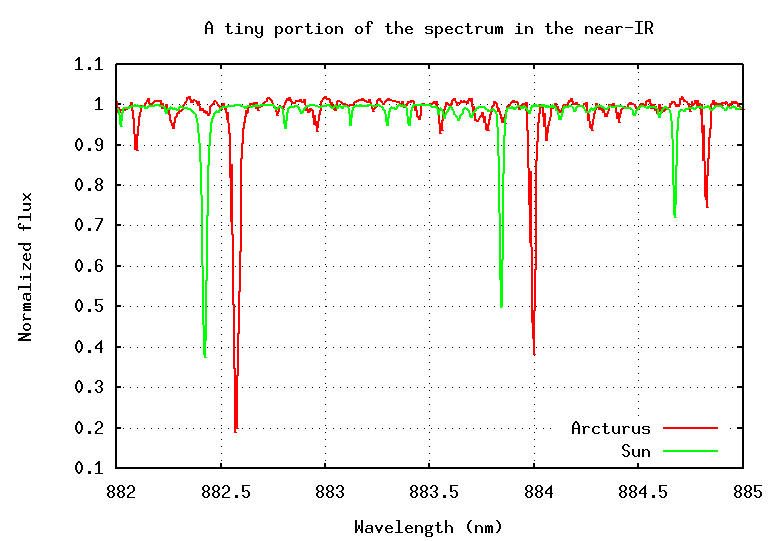
\includegraphics[width=0.5\textwidth]{images/spec_sun_arcturus}
	\caption{This image from Michael Richmond demonstrates the Doppler shift in spectra. \autocite{dopplerSpectroscopy}
	The shift is \( \lambda_{shift} = \lambda_{Arcturus} - \lambda{Sun} = \SI{882.55}{\nano\meter} - \SI{882.4}{\nano\meter} =  \SI{0.15}{\nano\meter}\).
	From that shift, \( v_{radial} = \frac{ \SI{0.15}{\nano\meter} }{ \SI{882.4}{\nano\meter} } \times \SI{3e8}{\kilo\meter\per\second} = \SI{50}{\kilo\meter\per\second} \)}
\end{figure}

While somewhat newer than the radial velocity method, the transit method has gained popularity in recent years
with the advent of missions such as Kepler, launched in 2009. The basic idea is to look for the slight drop
in the apparent brightness of a planet's host star as the planet passes between the star and Earth. Given that the
dimming effect is very small and can last for a short period of time, very sensitive instruments are needed,
and noise in the data is often a problem.\autocite{jplMethods} One advantage of this method is that
many stars can be observed at once, increasing the likelihood of detecting a planet, and Kepler
has detected more than 1,000 exoplanet candidates.\autocite{jplMethods}

To detect exoplanets using the transit method, a light curve plotting flux, or changes in intensity of the
light from the star, against time is generated from telescope images. A periodogram, which plots spectral density against frequency,
is then used to determine the period of the exoplanet. On the periodogram, peaks appear at frequencies corresponding
to the period. Once the period has been determined, further analysis of the light curve can determine the ingresses
and egresses of the transit. The transit depth, a measure of the difference in flux during and outside of a transit,
can be related to the radius of the planet:
\begin{align*}
	\Delta F &= \frac{ F_{\text{no transit}} - F_{\text{transit}} }{ F_{\text{no transit}} } \\
	&= (\frac{R_p}{R_*})^2
\end{align*}
This requires that the radius of the star, \(R_*\), is known in advance, but other methods can be used to determine this.
The BLS (Box-fitting Least Squares) algorithm is often used to search for transits, since it detects periodic differences
between two levels, i.e. the normal apparent brightness of the star and the decreased brighness during a transit.\autocite{bls}

For the purposes of this experiment, the transit method was chosen. This was largely due to the greater availability of data from the Kepler project,
but the transit method is also slightly simpler conceptually, which made it more suitable for a relatively straightforward implementation.
